\section{Aufgabe 2}
\subsection{Teilaufgabe a}
Die Gleichung
\begin{equation}
  \frac{d \sigma}{d \Omega}=\frac{\alpha ^2}{s} \cdot \left(\frac{2+\sin^2{\theta}}{1-\beta^2 \cdot \cos^2{\theta}} \right)
\end{equation}
mit
\begin{align}
  s=\left( 2E_e\right)^2 \\
  \beta=\sqrt{1-\gamma^{-2}} \\
  \gamma=\frac{E_e}{m_e} \\
  m_e= \SI{511}{keV}
\end{align}
ist numerisch nicht stabil. Dies lässt sich mit der Folge der vielen Operationen begründen. \\
Außerdem lässt sich in der ausgeschriebenden Form
\begin{equation}
  \frac{d \sigma}{d \Omega}=\frac{\alpha ^2}{4E^2_{e}} \cdot \left(\frac{2+\sin^2{\theta}}{1-\left(1-\frac{m_{e}}{E_{2}} \right) \cdot \cos^2{\theta}} \right)
\end{equation}
sehen, dass die Gleichung für den Fall $\theta = n \cdot \pi$, $n \in \mathbb{Z}$ besonders instabil ist , da
$\cos^2{\pm \pi}=1$ gilt und somit im Nenner  zwei gleichgroße Zahlen voneinander subtrahiert werden.
Zusätzlich findet im Fall $E_e=\SI{50}{GeV}$ eine Division durch eine kleine Zahl statt $\left( {\frac{m_{e}}{E_{2}}}^2 \ll 1 \right)$, womit die Gleichung numerisch instabil ist.


\subsection{Teilaufgabe b} \label{sec:2b}

\begin{align}
  \frac{d \sigma}{d \Omega} &= \frac{\alpha ^2}{s} \cdot \left(\frac{2+\sin^2{\theta}}{1-\beta^2 \cdot \cos^2{\theta}} \right) \\
  &=\frac{\alpha ^2}{s} \cdot \left(\frac{2+\sin^2{\theta}}{1-\beta^2 + \beta^2 \cdot \sin^2{\theta}} \right) \\
  &=\frac{\alpha ^2}{s} \cdot \left(\frac{2+\sin^2{\theta}}{\gamma^{-2} + \left(1-\gamma^{-2} \right) \cdot \sin^2{\theta}} \right) \\
  &=\frac{\alpha ^2}{s} \cdot \left(\frac{2+\sin^2{\theta}}{\gamma^{-2} \cdot \left(1-\sin^{2}{\theta} \right) + \sin^2{\theta}} \right) \\
  &=\frac{\alpha ^2}{s} \cdot \left(\frac{2+\sin^2{\theta}}{\gamma^{-2} \cdot \cos^2{\theta} + \sin^2{\theta}} \right)  \label{eqn:dwqsb}\\
\end{align}
Das Ergebnis ist numerisch stabiler, da die Substraktion zwei gleich großer Zahlen im Nenner vermieden wurde und sie durch die Addition von zwei quadrazischen Funktionen auch nicht mehr auftreten kann.

\subsection{Teilaufgabe c}
\begin{figure}[H]
  \centering
  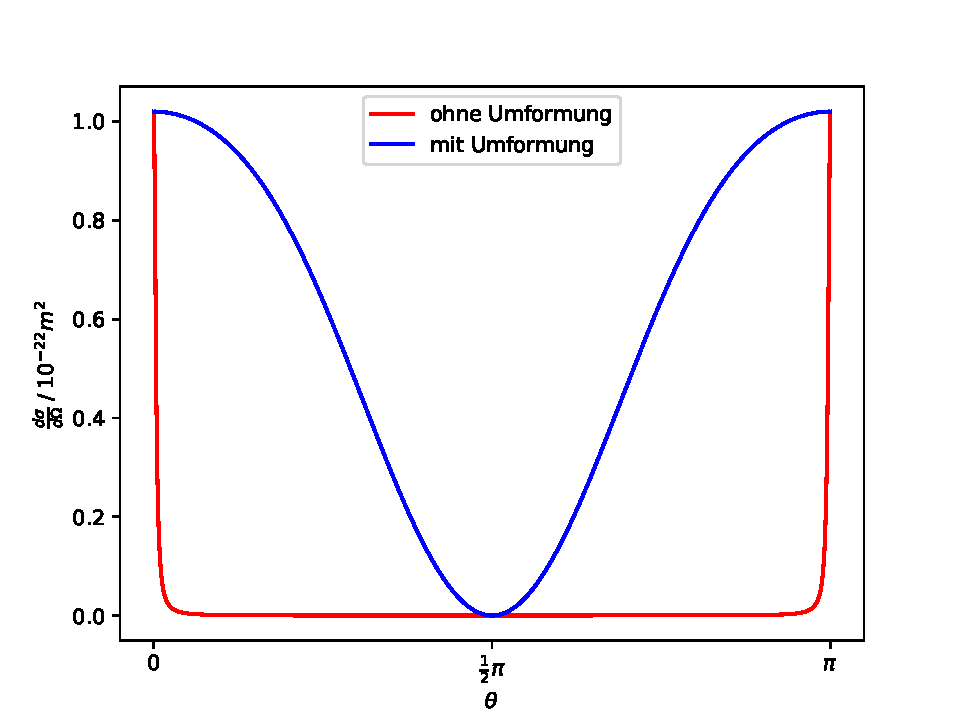
\includegraphics[width=\textwidth]{diffquerschnitt.pdf}
  \caption{Darstellung des differentiellen Wirkungsquerschnitts, mit und ohne die Umformung aus \ref{sec:2b} }
  \label{fig:2b}
\end{figure}
Wie in \ref{fig:2b} zu sehen ist, hebt sich die Kurve, die mit der Gleichung aus \eqref{eqn:dwqsb} berechnet wurde, deutlich von der anderen ab.
Statt einem Plateau ist nun eine parabelförmige Funktion zu sehen, woraus sich schließen lässt, dass dass die neue Funktion \eqref{eqn:dwqsb} numerisch stabiler ist.

\subsection{Teilaufgabe d} \label{sec:2d}
Die Konditionszahl ist definiert durch
\begin{equation}
  k=\mid \frac{f'(x)}{f(x)} \cdot x \mid
\end{equation}
\begin{align}
  f(\theta) &= \frac{\alpha ^2}{s} \cdot \left(\frac{2+\sin^2{\theta}}{1-\beta^2 \cdot \cos^2{\theta}} \right) \\
  f'(\theta) &= -\frac{a^2}{s} \cdot \frac{\cos{\theta} \sin{\theta} \cdot \left(3b^2-1 \right)}{\left (b^2\cos^2{\theta}-1 \right)^2} \\
  \rightarrow k &=  \frac{|\left( 3b^2-1\right) \theta \cdot \sin {\left(2 \theta \right)|}}{| \left(\sin^2{\theta}+2 \right) \cdot \left(\beta^2 \cdot \cos^2{\theta}-1 \right )| } \mid
\end{align}

\subsection{Teilaufgabe d}
\begin{figure}[H]
  \centering
  \includegraphics[width=\textwidth]{Konditionierungszahl.pdf}
  \caption{Darstellung der Konditionierungszahl k aus  \ref{sec:2d} }
  \label{fig:2d}
\end{figure}
Wie in Abbildung \ref{fig:2d} zu sehen ist, ist das Problem gut für $0<x<\pi$ konditioniert.
